\chapter{Results}
\label{ch:results}



% intro to results



% % % The model lines

\begin{table}[p]
    \centering
    \caption{
        The lines in the HyperSpy models for the GaAs sample, when As and Ga are added as elements.
        The dashed lines are the lines that are not used in the model, because of low overvoltage.
        HyperSpy differentiates between "X-ray lines" and "Family lines", where the first are the alpha lines of the element.
    }
    \label{tab:results:model_lines}
    \begin{tabular}{c|ccccccccccc}
        X-ray lines  &       &        &       &       &        &       &        &       &       &        \\
        % Model        &       &        &       &       &        &       &        &       &       &        \\
        30 kV        & As Ka & As La  & Ga Ka & Ga La &        &       &        &       &       &        \\
        15 kV        & As Ka & As La  & Ga Ka & Ga La &        &       &        &       &       &        \\
        10 kV        & ----- & As La  & Ga Ka & Ga La &        &       &        &       &       &        \\
        5            & ----- & As La  & ----- & Ga La &        &       &        &       &       &        \\
        \hline
        Family lines &       &        &       &       &        &       &        &       &       &        \\
        30 kV        & As Kb & As Lb1 & As Ln & As Ll & As Lb3 & Ga Kb & Ga Lb1 & Ga Ln & Ga Ll & Ga Lb3 \\
        15 kV        & As Kb & As Lb1 & As Ln & As Ll & As Lb3 & Ga Kb & Ga Lb1 & Ga Ln & Ga Ll & Ga Lb3 \\
        10 kV        & ----- & As Lb1 & As Ln & As Ll & As Lb3 & ----- & Ga Lb1 & Ga Ln & Ga Ll & Ga Lb3 \\
        5  kV        & ----- & As Lb1 & As Ln & As Ll & As Lb3 & ----- & Ga Lb1 & Ga Ln & Ga Ll & Ga Lb3
    \end{tabular}
\end{table}

% \begin{table}[p]
    \centering
    \caption{
        The estimated FWHM of Mn K$\alpha$ with different reference lines.
        When using 'all\_alpha', the alphabetically first line is used as reference.
        That is, for 30 and 15 kV, As K$\alpha$ is used as reference.
        For 10 and 5 kV, As L$\alpha$ is used as reference.
        The original resolution is from the instrument software.
    }
    \label{tab:results:estimated-FWHM}
    \begin{tabular}{ccccc}
        Reference line      & 30 kV & 15 kV & 10 kV & 5 kV  \\
        \hline
        original resolution & 130.0 & 130.0 & 130.0 & 130.0 \\
        \verb|'all_alpha'|  & 138.3 & 148.8 & 132.0 & 132.2 \\
        As Ka               & 137.9 & 146.4 & nan   & nan   \\
        As La               & 130.0 & 130.4 & 131.9 & 132.1 \\
        Ga Ka               & 132.9 & 131.7 & 668.3 & nan   \\
        Ga La               & 129.7 & 130.9 & 127.4 & 130.8
    \end{tabular}
\end{table}


% \subsection{Energy resolution}
% \label{results:resolution}


\section{Optimization of the acquisition parameters}
\label{results:acquisition_parameters}


\subsection{Process time}
\label{results:process_time}


One of the parameters which was tested was the process time.
The process time is a trade-off between the energy resolution and the throughput.
This effect is illustrated in \cref{fig:results:energy_resolutions_process_time}, which is a plot of the a GaSb spectrum at minimum and maximum process time for a SDD.
The figure have three panels, one for low, medium, and high energy X-rays.
The effect of the lowered energy resolution is most prominent for the low energy X-rays, but the effects is most dependent on what lines are present in the spectrum.
The difference between the peak centers and theoretical line energies in panel (a) is due to the poorer calibration at low energies.
Data was acquired with process time 2 and 4 too (not shown), which is included in talbe \dots


% figures eds_energyResolutions_process_time.pdf
\begin{figure}[hptb]
    \centering
    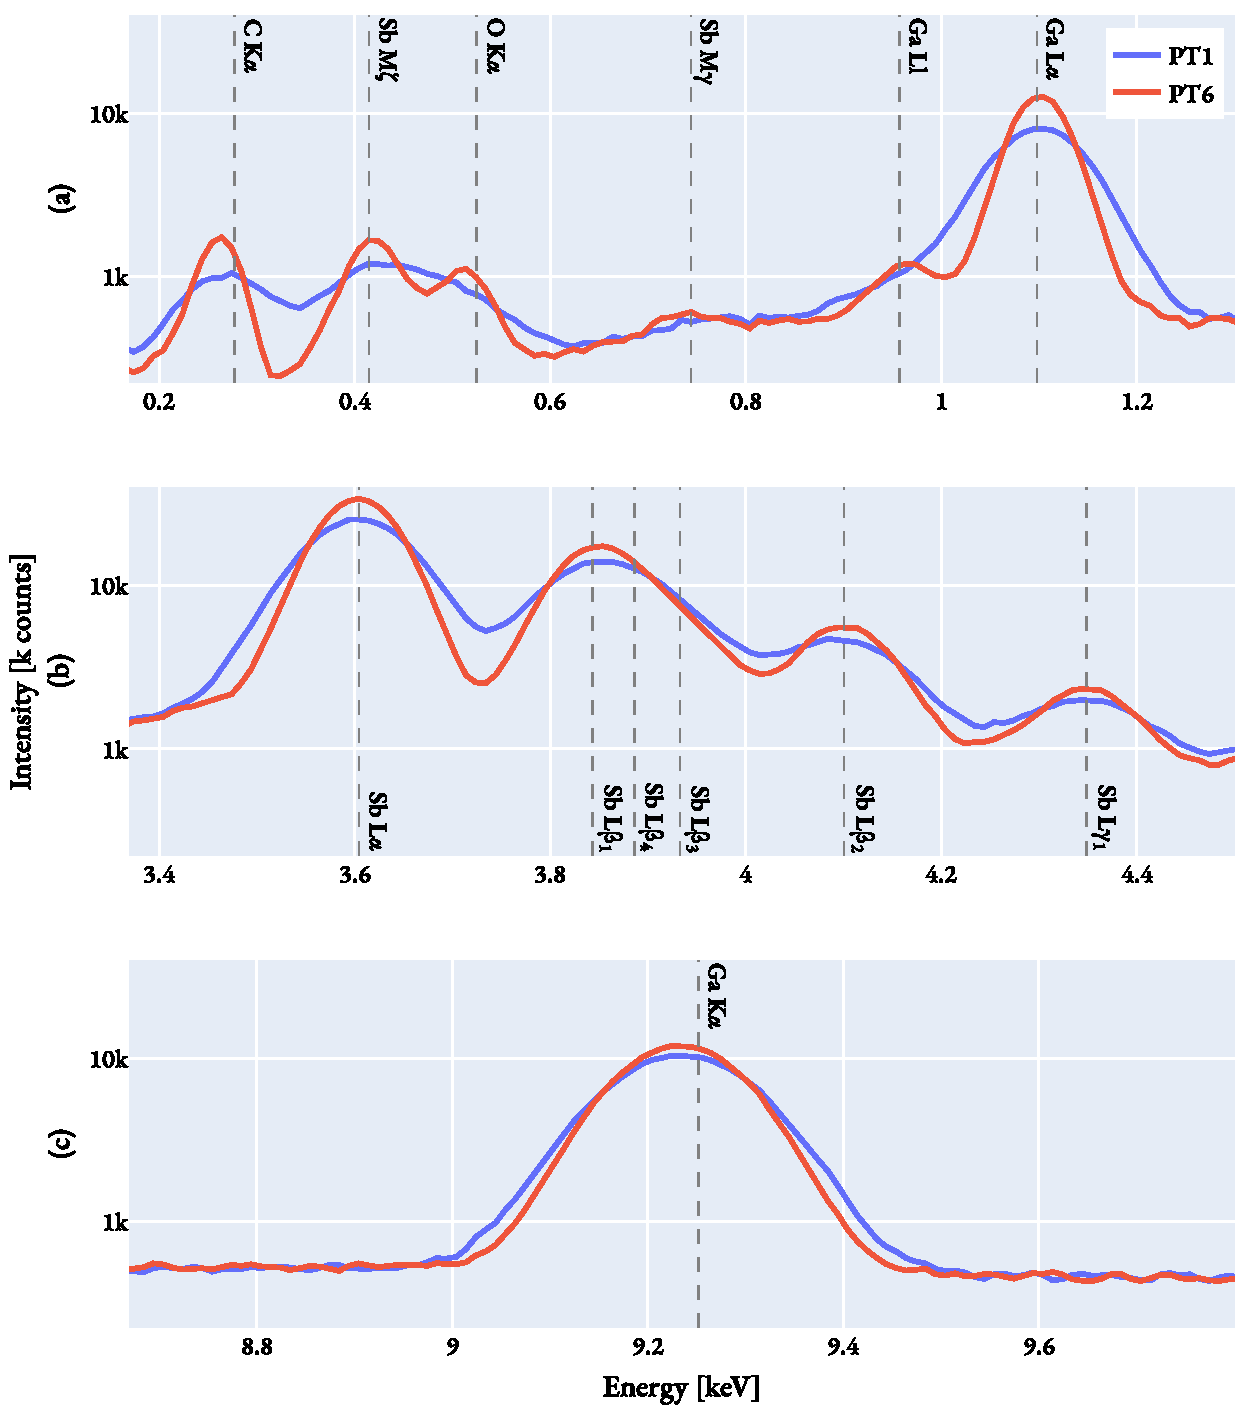
\includegraphics[width=0.95\linewidth]{figures/results/eds_energyResolutions_process_time.pdf}
    \caption{
        Illustration of different energy resolutions on the same specimen, because of different process times.
        The maximum (red) and minimum (blue) process time (PT) on the instrument is used.
        Panel (a) is the spectrum at low energy, where the effect most influential.
        Here both the Sb M$\eta$ and O K$\alpha$, and the Ga Ll and Ga L$\alpha$ are overlapping too much with PT1.
        Panel (b) is the spectrum at medium energy, where the effect less influential.
        Panel (c) is the spectrum at high energy, where the effect is almost negligible.
        All three panels span 1.13 keV and have the same range of counts.
        The vertical lines are the theoretical line energies.
    }
    \label{fig:results:energy_resolutions_process_time}
\end{figure}
